\section{Regiones}

Desde 2007, geográficamente Chile está dividido en 16 regiones desde Arica hasta la Antártica Chilena. Además de la división geográfica, también existen las regiones naturales (zonas), las cuales son cinco:

\begin{tasks}[label =$\bullet$](4)
    \task Norte Grande \\
    \task Zona Central \\
    \task Zona Austral \\
    \task Norte Chico \\
    \task Zona Sur
\end{tasks}
\vglue5mm

La tarea que se le encomienda a Ud., es construir ciertas funciones que ayuden a obtener información con respecto a estas divisiones. Para esto, Ud. cuenta con la información de cada región en el archivo \texttt{regiones.txt}, donde en cada línea se encuentra el número de la región, el nombre, la cantidad de habitantes, la superficie (en km2) y la capital; es importante saber que las regiones están ordenadas de manera ascendente según su número. Por otro lado, Ud. cuenta con la información de cada región natural en el archivo \texttt{zonas.txt}, en el cual cada línea se encuentra la zona natural junto con las regiones que pertenecen a ella.

%\input{Figures/f1.tex}
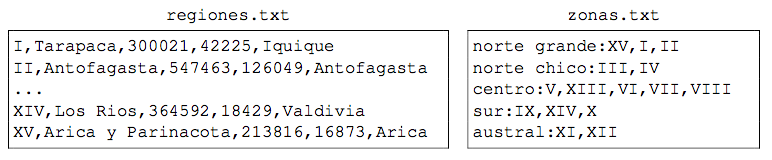
\includegraphics[width=15cm]{Images/f1.png}

Defina claramente (indicando las parámetros de la función) y desarrolle las funciones que solucionen la siguientes interrogantes:
\begin{enumerate}[label=\alph*)]
    \item Con un archivo del tipo \texttt{zonas.txt}, retorne un diccionario, donde la llave sea la zona y el valor sea una lista con las regiones que la forman.
    \item Con un archivo del tipo \texttt{regiones.txt} y otro del tipo \texttt{zonas.txt}, retorne un diccionario, donde la llave sea la zona y el valor sea la cantidad de habitantes para tal zona.
    \item Después de la 3ra guerra mundial, el páıs ha sufrido modificaciones en su geografía, por supuesto a su favor, por lo que es necesario actualizar tanto el archivo \texttt{regiones.txt} como $\texttt{zonas.txt}$. Se debe agregar a ambos archivos la(s) nueva(s) región(es) que ha ganado el páıs con la información entregada: nombre de la región, superficie (en km2), habitantes, capital y a la región natural que va a pertenecer.
\end{enumerate}

Nota: cada vez que se agrega una región, le corresponde el número que sigue; por ejemplo la primera región en agregar será la decimosexta región. Asuma que existe la función \texttt{entero\_a\_romano(x)} que convierte el entero \texttt{x} a número romano.

%\begin{lstlisting}[style=consola]
%>>>funcion(2)
%4
%\end{lstlisting}